\documentclass[a4paper,11pt]{article}
\usepackage[margin=2cm]{geometry}
\usepackage[T1]{fontenc}
\usepackage[utf8]{inputenc}
\usepackage{lmodern}
\usepackage{graphicx}
\usepackage{enumitem}
\usepackage{hyperref}
\setlist{nosep}
\setlength{\parindent}{0pt}
\setlength{\parskip}{.65em}
\newcommand{\intellicart}{Intellicart}
\newcommand{\file}[1]{\texttt{#1}}

\title{INTELLICART CARTRIDGE\\USER MANUAL}
\author{Cartheur Research}
\date{}

\begin{document}
\maketitle

The hardware cartridge ``Intellivision \intellicart'' (henceforth referred to as Intellicart) allows Program/Game files to be loaded on an Intellivision console. These files are ``Cartridge Dumps'': transfers of programs contained in Intellivision-cartridge ROMs. Store the files on a micro SD card, insert it in the compartment on the left of the Intellicart, then insert the Intellicart into the console cartridge port.

\section*{Technical features}
\begin{itemize}
  \item Supported console: Mattel Intellivision.
  \item Compatible files: \file{.BIN} + \file{.CFG}.
  \item Reads files from a micro SD card; compatible media are 1--32~GB micro SD cards formatted FAT or FAT32.
  \item Compatible with PAL, NTSC, and SECAM Intellivision consoles.
  \item Files are searched and loaded using the three push buttons on the cartridge.
  \item Place titles in the micro SD root, or in folders in that root; subfolders cannot be used.
  \item Store the basic \file{0.cfg} configuration file in the root; see the appendix.
  \item Long names are supported up to 45 characters plus the file extension.
  \item The OLED displays folders and files. Two LEDs indicate cartridge operation.
  \item Power is supplied directly from the console cartridge port.
\end{itemize}

\section*{Important}
Make all electrical and mechanical connections or disconnections with equipment switched off and cables disconnected from mains outlets.

Clean the Intellicart only with antistatic cloths; do not use liquids. It contains electronic components and a PLA or ABS plastic case. Do not press the small OLED-display window: it is delicate and pressure can damage or dislodge it, damaging internal components. Do not disassemble the cartridge or attempt repairs; only qualified personnel should do so.

Do not spill liquids on the Intellicart. After an accidental spill, do not insert it into the console; if it is already inserted, immediately unplug the console. Dry and clean the Intellicart completely before connecting it.

The user is solely responsible for damage to people, animals, or property arising from use of the Intellicart cartridge. Cartheur Research, B.V., the hardware designer, manual author, and vendors are not responsible for such damage. Using the Intellicart Cartridge for Intellivision signifies agreement to these conditions.

\section*{Intellivision console connection}
Insert the cartridge directly into the console's right cartridge port, with the side containing the text and LEDs facing up.

\textit{Tip:} Place a stand or support base under the Intellicart so it remains rigid while the push buttons are pressed. This prevents the cartridge from flexing and avoids force on the Intellivision connector contacts. Flexing can create false contacts, malfunctions, or eventually damage the console connector or cartridge. This is advisable because the Intellicart's buttons are on the cartridge itself.

\section*{Using the Intellicart cartridge}
On a personal computer (these directions assume Windows), copy program files with \file{.BIN} and \file{.CFG} extensions to the micro SD card. You may create folders only in the root to sort files by genre, type, and so on; do not create subfolders. Files may be in the root or one root-level folder. A \file{.BIN} must always have a same-named \file{.CFG}, for example \file{Burgertime.bin} and \file{Burgertime.cfg}.

\textit{Note:} If only the \file{.BIN} file is transferred, Intellicart uses the default configuration \file{0.cfg}, which must be in the SD-card root. It may or may not be compatible with that \file{.BIN}. In general, \file{0.cfg} works with most, but not all, ROMs. If neither the associated configuration nor \file{0.cfg} is present, the Program/Game cannot run.

The \file{.BIN} contains the ROM dump; the \file{.CFG} tells the cartridge how its data areas are allocated in the Intellivision memory map. Without correct configuration data, Intellicart does not know where to place ROM contents and cannot start the program.

Some \file{.CFG} files contain ``Hacks'', such as infinite lives, longer stages, invulnerability, or a starting-stage selection. When Intellicart detects them, it asks whether to activate them. Press PB~2 to activate Hacks; press PB~1 or PB~3 to start the standard game. Emulator-oriented Hack configurations may not be fully compatible with the console and Intellicart.

\textit{Tip:} To retain alphabetical OLED order, keep all Programs/Games in a PC folder. Select all titles and folders, copy starting from the first alphabetically, and paste them onto the SD card. To add titles later, add them first to that PC folder, erase the SD-card contents, then transfer the complete folder again. Adding files directly to a populated SD card can make new titles appear first or among existing titles.

\section*{Naming files}
Although long names are supported, simplify them to avoid a title not being recognized. Avoid spaces where practical; use hyphens and underscores instead. Avoid dots, apostrophes, commas, exclamation/question marks, asterisks, and similar symbols. Keep names under 45 characters.

For example, reduce \file{Masters of the Universe-The Power of He-Man! (1983) (Mattel).bin} to \file{Masters\_o\_t\_Universe-T\_P\_o\_He-Man-(1983).bin}. You may retain original names if desired, provided they meet the length limit. Simplification is needed only if a title appears as a blank space while browsing the OLED.

Once the card is prepared, insert it in the Intellicart's left-side slot with its label facing up and contacts facing down. Insert the Intellicart in the console's right cartridge slot, then turn on the television/monitor and console.

\section*{Intellicart push-button functions}
\begin{center}
  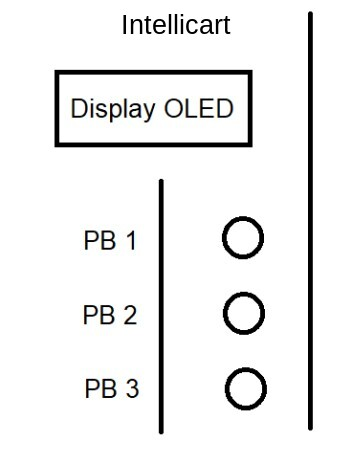
\includegraphics[width=.38\textwidth]{user-manual-asset-000.jpg}
\end{center}

\subsection*{Before starting a ROM}
\begin{description}[style=nextline]
  \item[PB 1] Scroll titles and folders forward.
  \item[PB 2] Enter or exit a folder; start the selected file. To exit a folder, use PB~1 or PB~3 to show either \file{. . Kb:0} exit point, then press PB~2.
  \item[PB 3] Scroll titles and folders backward.
\end{description}

\subsection*{While a Program/Game is running}
\begin{description}[style=nextline]
  \item[PB 1] Reset the Intellivision. If the TV/monitor becomes black, the console's reset-line capacitor is defective; also press the console Reset button to restart the running program.
  \item[PB 2] Not used.
  \item[PB 3] Reset the Intellicart cartridge.
\end{description}

When powered on, the TV/monitor shows \texttt{Intellicart - Cart Please Select a Game}; the OLED shows \texttt{Press a Button on Intellicart}. Use PB~1 and PB~3 to select titles or folders. If the main screen does not appear and navigation does not work, the console's reset-line capacitor is defective. Press the Intellivision Reset button to activate Intellicart and show the main screen.

PB~2 enters a folder or starts a Program/Game. The OLED displays \file{filename.bin}, not the system-only \file{filename.cfg}, and shows ROM size in Kb beneath it. Pressing PB~2 loads the ROM and shows \texttt{Emulating ROM: filename.bin}. If the display remains black because of the defective capacitor, press the console Reset button to start the Program/Game.

Once started, control moves to the Intellivision gamepads. The console Reset button or Intellicart PB~1 restarts the Program/Game as if an original cartridge were inserted. PB~3 resets Intellicart and unloads the game; the OLED returns to \texttt{Press a button on Intellicart} and the TV/monitor goes black. With the defective capacitor, press the console Reset button after unloading before selecting another Program/Game.

\section*{Intellivision file formats}
The three common cartridge-dump formats are \file{filename.BIN}, \file{filename.INT}, and \file{filename.ROM}.
\begin{enumerate}
  \item \file{filename.BIN} is the classic binary ROM dump and requires \file{filename.CFG}.
  \item \file{filename.INT} is the same binary format with a different extension, originally used by emulators to avoid Windows \file{.BIN} associations. It also requires \file{filename.CFG}.
  \item \file{filename.ROM} includes both binary and configuration data, so it does not need a separate configuration file.
\end{enumerate}
Intellicart supports only \file{.BIN}; \file{.INT} and \file{.ROM} will not appear on the OLED and are not handled directly.

\subsection*{\file{filename.INT}}
Rename the extension from \file{.INT} to \file{.BIN}, for example \file{burgertime.int} becomes \file{burgertime.bin}, then treat it as an ordinary BIN file.

\subsection*{\file{filename.ROM}}
A ROM file embeds the corresponding BIN and CFG data. Extract them using \file{rom2bin.exe}, available in the \texttt{bin/} directory of the jzIntv SDK at \url{http://spatula-city.org/~im14u2c/intv/}. Copy \file{rom2bin.exe} and the files to convert into one folder, then drag \file{namefile.rom} onto \file{rom2bin.exe}. This produces \file{namefile.bin} and \file{namefile.cfg}, which are compatible with Intellicart.

\section*{If a Program/Game does not run}
\begin{enumerate}
  \item BIN and CFG names differ. Rename the CFG to match the BIN exactly.
  \item Files are in a subfolder. Move them to the SD-card root or a root-level folder, then delete the subfolder.
  \item A ROM was converted incorrectly. Repeat the conversion.
  \item The BIN is not an Intellivision binary ROM. It is unusable.
  \item The BIN or CFG is corrupt. It is unusable.
  \item The CFG is incorrect or emulator-only. Correct and edit the CFG.
\end{enumerate}

\section*{Correcting and editing CFG files}
CFG files originated for Intellivision emulators and define ROM/RAM memory allocation. Emulator evolution has added parameters, so multiple CFG variants may exist for one game. Intellicart recognizes basic mappings. For example, the first version below works, while the second must have its \texttt{ECS} line removed.
\begin{verbatim}
[mapping]                 [mapping]
$0000 - $1FFF = $5000     ECS
                          $0000 - $1FFF = $5000
\end{verbatim}

Example standard configuration:
\begin{verbatim}
[mapping]
$0000 - $1FFF = $5000 ; 8K to $5000 - $6FFF
$2000 - $2FFF = $D000 ; 4K to $D000 - $DFFF
$3000 - $3FFF = $F000 ; 4K to $F000 - $FFFF
\end{verbatim}

A Hack configuration can add sections after the mapping:
\begin{verbatim}
[mapping]
$0000 - $1FFF = $5000
[memattr]
$D000 - $DFFF = ROM 16
$F000 - $FFFF = ROM 16
[macro]
p 633a 34 ; Infinite peppers (both players)
p 51f9 34 ; Infinite lives (both players)
\end{verbatim}

No text or parameters may occur before \file{[mapping]}; delete any that do. Complex emulator CFGs may contain \file{[vars]} metadata before mapping and must be trimmed so that \file{[mapping]} begins the file. Retain the mapping, memory attributes, and desired macro lines.

To edit \file{filename.cfg} on Windows, temporarily add \file{.TXT}, producing \file{filename.cfg.txt}; accept Windows' extension-change warning. Open it in a text editor such as Notepad, edit and save it, then remove the added \file{.TXT} extension before testing.

\section*{Appendix: basic \file{0.cfg}}
Find \file{0.cfg} online or create it in a text editor with the following contents, then save it as \file{0.cfg}:
\begin{verbatim}
[mapping]
$0000 - $1FFF = $5000 ; 8K to $5000 - $6FFF
$2000 - $2FFF = $D000 ; 4K to $D000 - $DFFF
$3000 - $3FFF = $F000 ; 4K to $F000 - $FFFF
\end{verbatim}

\end{document}
